\section{Design and Simulation}

\begin{figure}[h]
    \centering
    
    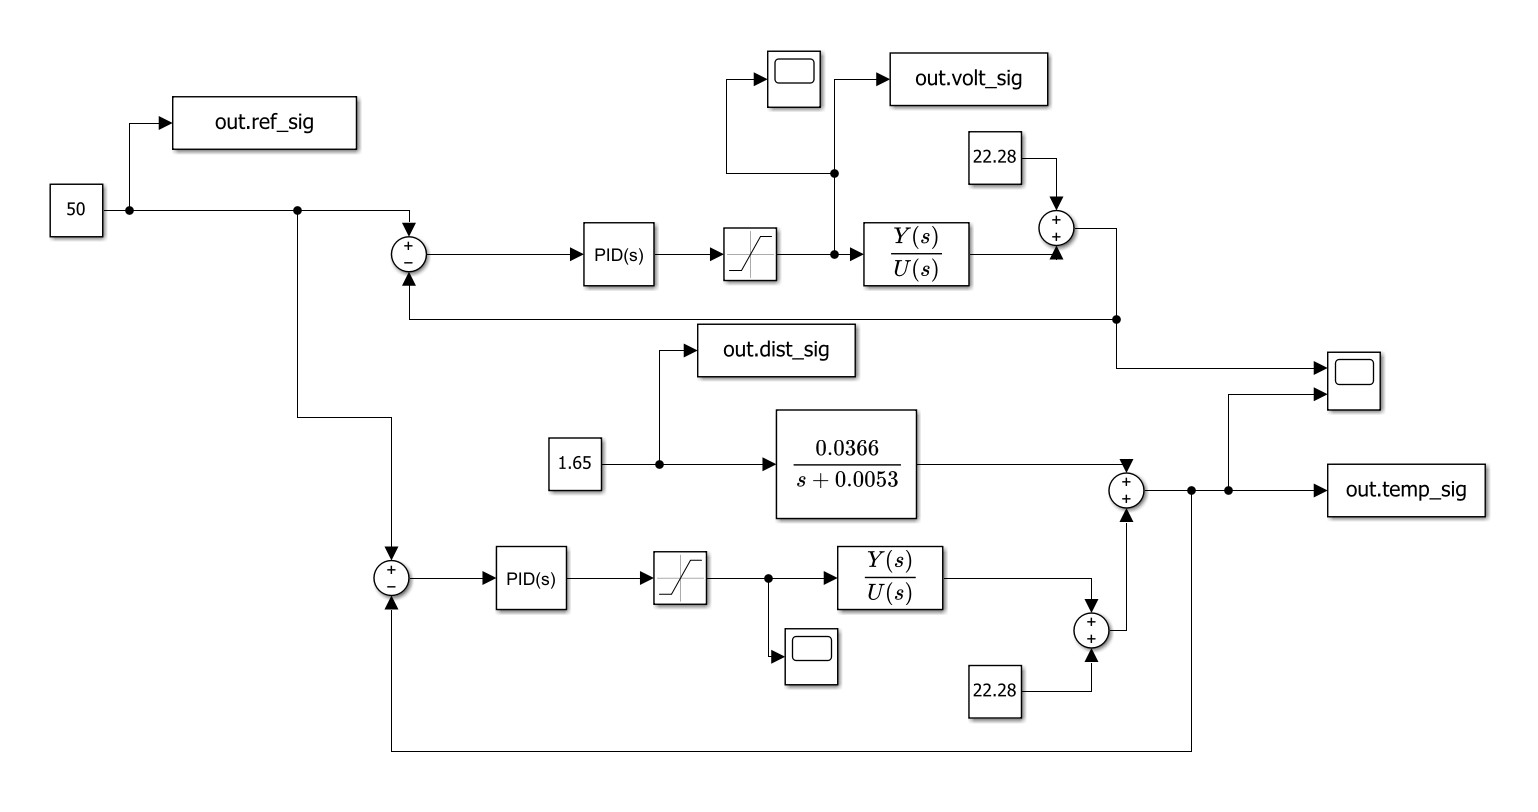
\includegraphics[width=0.9\textwidth]{Images/Disturb_reject_model.jpg}
    \caption{Simulink model for the disturbance rejection PID controller.}
    \label{fig:simulink_dr}
\end{figure}

\begin{table}[h]
    \centering
    \caption{Controller parameters and closed-loop step response metrics. (Open-loop baseline: $t_r = 289.08$s, $t_p = \infty$, $t_s = 514.747$s, Overshoot = 0\%). See Figure \ref{fig:all_step_responses} for the corresponding step response graphs.}
    \vspace{2mm}
    
    \begin{tabular}{@{} m{3.5cm} m{4cm} m{6cm} @{}}
        \toprule
        \textbf{Controller} & \textbf{Parameters} & \textbf{Closed-Loop Metrics} \\
        \midrule
        
        \textbf{P-Control} & 
        $K_p = [val]$ & 
        Rise Time: [val]s \newline Peak Time: [val]s \newline Settling Time: [val]s \newline Overshoot: [val]\% \\
        \midrule
        
        \textbf{PI-Control} & 
        $K_p = [val]$ \newline $K_i = [val]$ & 
        Rise Time: [val]s \newline Peak Time: [val]s \newline Settling Time: [val]s \newline Overshoot: [val]\% \\
        \midrule

        \textbf{PD-Control} & 
        $K_p = [val]$ \newline $K_d = [val]$ & 
        Rise Time: [val]s \newline Peak Time: [val]s \newline Settling Time: [val]s \newline Overshoot: [val]\% \\
        \midrule
        
        \textbf{PID-Control} \newline (Reference) & 
        $K_p = [val]$ \newline $K_i = [val]$ \newline $K_d = [val]$ & 
        Rise Time: [val]s \newline Peak Time: [val]s \newline Settling Time: [val]s \newline Overshoot: [val]\% \\
        \midrule

        \textbf{PID-Control} \newline (Disturbance) & 
        $K_p = 0.067424$ \newline $K_i = 0.0016631$ \newline $K_d = 0.68337$ & 
        Rise Time: 102.934s \newline Peak Time: 225.625s \newline Settling Time: 366.913s \newline Overshoot: 9.26\% \\
        
        \bottomrule
    \end{tabular}
    \label{tab:controller_comparison}
\end{table}

\clearpage % Forces the figure onto a new, dedicated page

\begin{figure}[h!]
    \centering
    
    % Graph 1: P
    \begin{subfigure}[b]{0.45\textwidth}
        \centering
        % \includegraphics[width=\textwidth]{graphs/P_step.pdf}
        \caption{P-Control}
    \end{subfigure}
    \hfill
    % Graph 2: PI
    \begin{subfigure}[b]{0.45\textwidth}
        \centering
        % \includegraphics[width=\textwidth]{graphs/PI_step.pdf}
        \caption{PI-Control}
    \end{subfigure}
    
    \vspace{0.5cm} % Adds breathing room between rows
    
    % Graph 3: PD
    \begin{subfigure}[b]{0.45\textwidth}
        \centering
        % \includegraphics[width=\textwidth]{graphs/PD_step.pdf}
        \caption{PD-Control}
    \end{subfigure}
    \hfill
    % Graph 4: PID Reference
    \begin{subfigure}[b]{0.45\textwidth}
        \centering
        % \includegraphics[width=\textwidth]{graphs/PID_ref_step.pdf}
        \caption{PID-Control (Reference Tracking)}
    \end{subfigure}
    
    \vspace{0.5cm}
    
    % Graph 5: PID Disturbance 
    \begin{subfigure}[b]{0.45\textwidth}
        \centering
        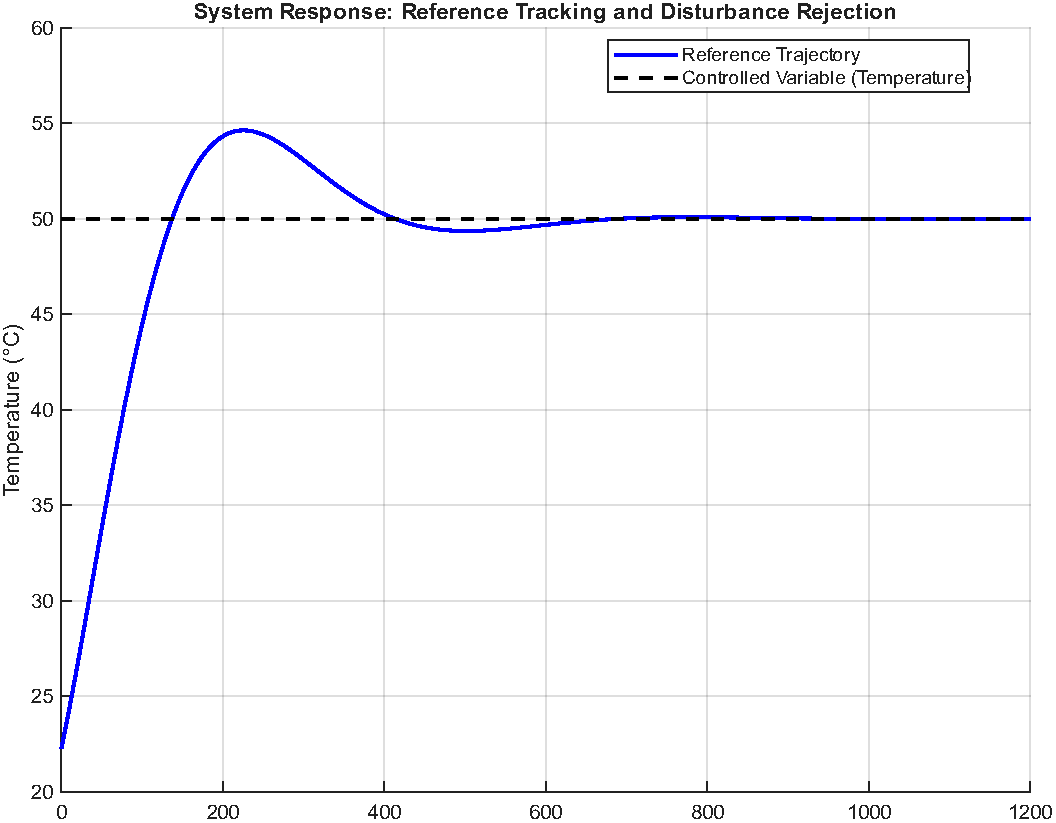
\includegraphics[width=\textwidth]{Images/PID_dist_reject_closed_loop.pdf}
        \caption{PID-Control (Disturbance Rejection)}
    \end{subfigure}
    
    \caption{Open-loop vs closed-loop step responses for all controller configurations.}
    \label{fig:all_step_responses}
\end{figure}

\todo[inline, color=yellow]{Move these figures around as needed, I just placed them here for now.}


\clearpage % Forces everything after this onto a new page

\begin{figure}[p]
    \centering
    
    % Graph 1: Without Disturbance
    \begin{subfigure}[b]{0.9\textwidth}
        \centering
        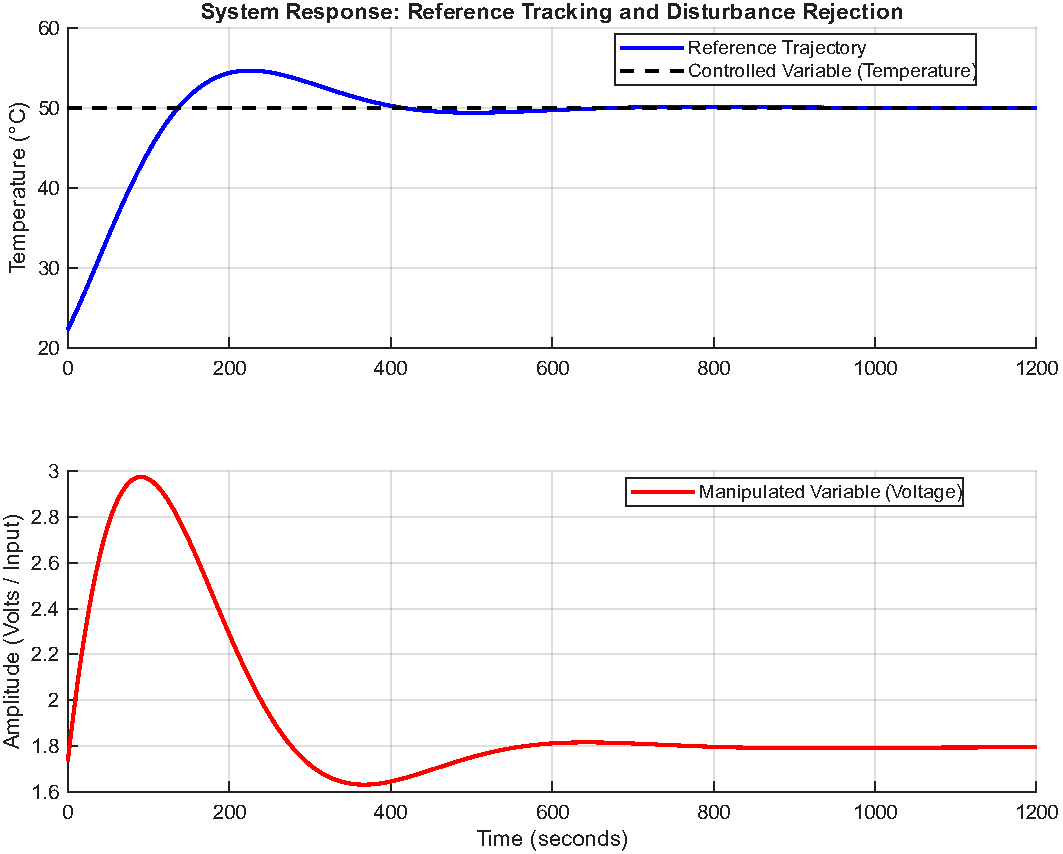
\includegraphics[width=\textwidth, height=0.4\textheight, keepaspectratio]{Images/PID_Dist_Reject_no_dist.pdf}
        \caption{Closed-loop response (No Disturbance).}
        \label{fig:sim_no_dist}
    \end{subfigure}
    
    \vspace{0.5cm} % Reduced from 1cm to save vertical space
    
    % Graph 2: With Disturbance
    \begin{subfigure}[b]{0.9\textwidth}
        \centering
        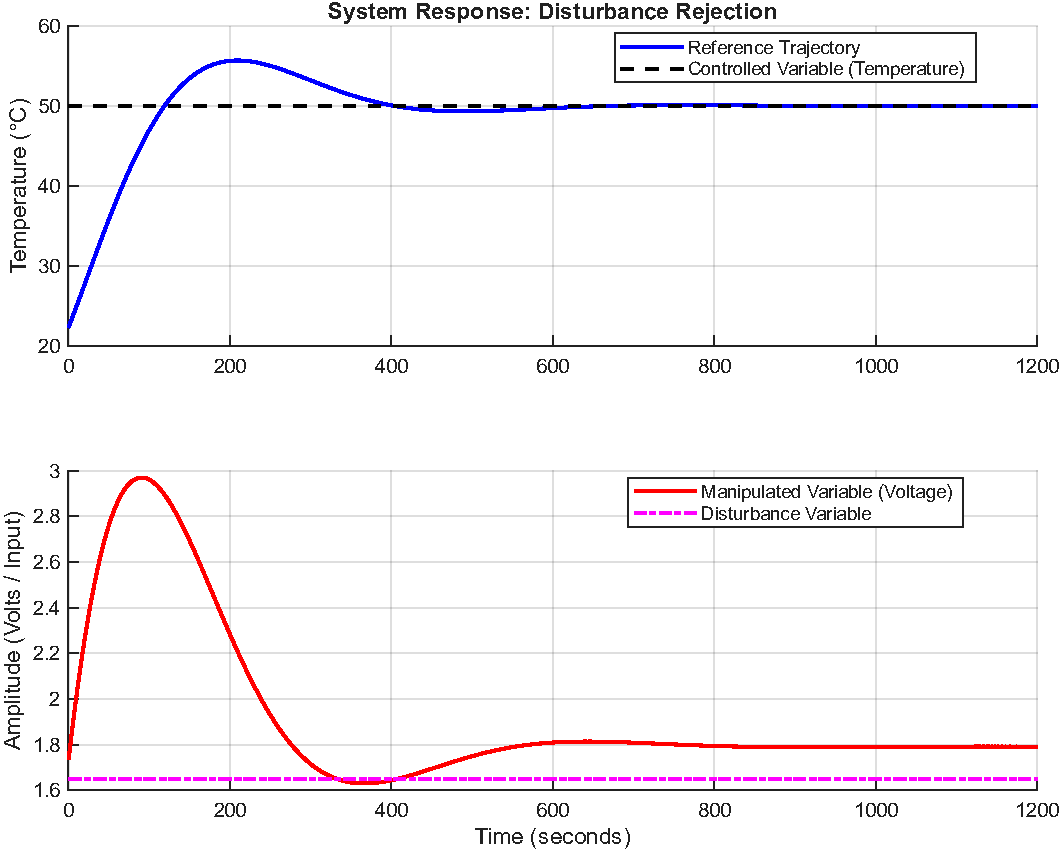
\includegraphics[width=\textwidth, height=0.4\textheight, keepaspectratio]{Images/PID_dist_reject_dist.pdf}
        \caption{Closed-loop response (50\% PWM Disturbance).}
        \label{fig:sim_with_dist}
    \end{subfigure}
    
    \caption{Simulink closed-loop step response for the disturbance-rejection PID controller. The bottom figure demonstrates the controller compensating for the external heat disturbance caused by transistor 2.}
    \label{fig:sim_disturbance_comparison}
\end{figure}

\clearpage


